\documentclass[
	fullscreen=true, 
	bookmarks=false,
	sans serif,
	9pt,
	pdf,
	hyperref={
		pdfpagelabels=false,
		unicode=true
	}
]{beamer}

\usepackage[utf8]{inputenc}
\usepackage[T2A]{fontenc}
\usepackage[english,russian]{babel}
\usepackage{pgfpages}
\pgfpagesuselayout{resize to}[a4paper,landscape,border shrink=0mm]

\usepackage{array}
\usepackage{epsfig}
\usepackage{epstopdf}
\usepackage{multirow}
\usepackage{listings}
\usepackage{tikz}
\usepackage{graphicx}

\lstset{
	tabsize=4,
	gobble=12,
	keepspaces=true,
	basicstyle=\normalsize\ttfamily,
	breaklines=true,
	columns=fullflexible,
}

\usetheme{Madrid}
% =====================================================================
% Info
\title{
	Исследование и разработка методов и алгоритмов анализа рентгеновских снимков лёгких для поиска последствий заболевания
}
\author{
	\vspace{0.5cm}\\
    Сажникова О.В.\\
	\vspace{0.1cm}
	ПИмд-11\\
	\vspace{2cm}
}
\institute{УлГТУ}
\date{08.12.2021}
% =====================================================================
% Document
\begin{document}
	
	% Title
	\begin{frame}
		\titlepage
	\end{frame}	
	% =====================================================================
		
	\section{}
	\subsection{}
		
	\begin{frame}\frametitle{Цель, объект и предмет исследования}
		Цель: улучшить качество распознавания заболеваемости по рентгеновским снимкам легких человеками с помощью нейронной сети.
		\newline
		
		Объект: Распознавание болезни легких человека: covid-19, пневмония, туберкулез.
		\newline
		
		Предмет: Нейронная сеть для распознавание болезни легких человека по рентгеновским снимкам.
	\end{frame}

	\begin{frame}\frametitle{Задачи и методы исследования}
	
		Определены следующие задачи исследования:
		\begin{itemize}
			\item Изучить предметную область;
			\item Сгенерировать обучающую выборку;
			\item Определить модель и архитектуру нейронной сети;
			\item Обучить нейронную сеть;
			\item Оценить результаты и сделать выводы.
			\newline
		\end{itemize}
	
		\newline
		
		Выявлены методы исследования:
		\begin{itemize}
			\item Теоретический;
			    \begin{itemize}
			        \item Метод сравнительного анализа: сравниваются несколько моделей нейронных сетей, которые обучаются на одинаковой выборке;
			    \end{itemize}
			\item Эмпирический;
			    \begin{itemize}
			        \item метод эксперимента: при определенных данных, метриках, скорости обучения, количествах эпох нейронная сеть обучается. После обучения у модели есть потери и точность при обучении, зафиксировав которые модель можно переобучить, изменив входящие параметры;
			    \end{itemize}
		\end{itemize}
	\end{frame}

	\begin{frame}\frametitle{Научная новизна}
		Научная новизна исследования состоит в том, что определен метод определения последствий заболевания: covid-19, пневмония, туберкулез, - на основе распознавания нейронной сетью рентгеновского снимка легких человека и его биологических данных. 
	\end{frame}

	\begin{frame}\frametitle{Положения, выносимые на защиту}
		Положения, выносимые на защиту:
		\begin{itemize}
			\item В ходе научного исследования выявлено, что большое количество поставленных диагнозов оказываются неверными по тем или иным причинам;
			\item Выявлена взаимосвязь между рентгенограммой легких и биологическими данными человека: при пограничном случае постановки диагноза между двумя заболеваниями данные пациента прямо влияют на выбор одного из диагнозов;
			\item Использование метода распознавания болезни по рентгенограмме легких с помощью нейронной сети и с учетом биологических данных человека повысит точность постановки диагноза и уменьшит количество ошибок.
			\newline
		\end{itemize}
	\end{frame}

	\begin{frame}[fragile]\frametitle{Статьи}	
		Н.Я. Лукьяненко, Я.Н. Шойхет «Сравнительные аспекты врачебных ошибок в диагностике больных с пневмониями и центральным раком легких»
А.Г. Волков, С.И. Пужаев «Ошибки при визуальной оценке рентгенограмм у больных параназальными синуситами»

        \begin{table}[]
            \begin{tabular}{|l|c|l|l|l|}
                \hline
                \multicolumn{1}{|c|}{Врачебные ошибки}        & Процент   \\ \hline
                Неправильная интерпретация клинических данных & $\sim$30\%  \\ \hline
                Недостаточная квалификация врача              & $\sim$30\%  \\ \hline
                Низкое качество рентгенограмм                 & $\sim$19\%   \\ \hline
            \end{tabular}
        \end{table}
        
        По итогу около 30 процентов поставленных диагнозов были неверными по разным причинам, основными из них это недостаточная квалификация врача, неправильная интерпретация данных и низкое качество рентгенограмм.

	\end{frame}
	
	\begin{frame}[fragile]\frametitle{Статьи}	
		S.V. Aksenov, K.A. Kostin, A.V. Ivanova, J. Liang, A.V. Zamyatin «An Ensemble of Convolutional Neural Networks for the Use in Video Endoscopy»
D. Y. Manylov «CURRENT DIRECTIONS IN THE DEVELOPMENT OF NEURAL NETWORKS»

Для решения проблем была разработана архитектура, в которой каждый нейрон связан только с небольшой областью изображения, а все нейроны имеют одинаковые веса. Этот процесс представляет собой свертку изображения. Отсюда пошли сверточные нейронные сети.

        \begin{figure}[h]
            \centering
            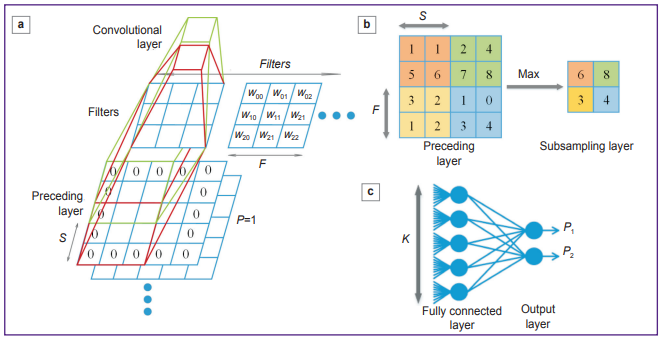
\includegraphics[width=0.50\textwidth]{img/picture_1.png}
            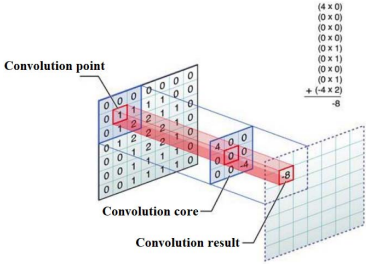
\includegraphics[width=0.30\textwidth]{img/picture_2.png}
        \end{figure}

	\end{frame}
	
	\begin{frame}[fragile]\frametitle{Статьи}	
		А.Д. Кульневич, Н.Д. Сергеева, Р.А. Чугунов «СИСТЕМА РАННЕГО ДЕТЕКТИРОВАНИЯ ПНЕВМОНИИ НА ОСНОВЕ МЕТОДОВ ГЛУБОКОГО ОБУЧЕНИЯ»

Авторы использовали нейронную сеть Masc R-CNN со следующими нововведениями:

1.	Для улучшения качества распознавания используется предобучение на изображениях набора данных Common Objects in Context (COCO)


2.	Для улучшения сходимости алгоритма коэффициент обучения изменяется циклично
После получения итогов были сделаны выводы, что точность распознавания таким алгоритмом ниже, чем медицинскими экспертами.

	\end{frame}
	
	\begin{frame}[fragile]\frametitle{Статьи}	
		А. А. Арбузова «ДИАГНОСТИКА ПНЕВМОНИИ ПО РЕНТГЕНОВСКИМ СНИМКАМ С ПОМОЩЬЮ СВЕРТОЧНЫХ НЕЙРОННЫХ СЕТЕЙ»

Функция потерь в виде функции бинарной перекрестной энтропии (binary-crossentropy):

        \begin{equation}
          H_{p}(q) = - \frac{1}{N}\sum\limits_{i=1}^N y_{i}\log_2 p(y_{i}) + (1-y_{i}) \log_2 (1-p(y_{i})) ,
        \end{equation}
        
    Результаты экспериментов:
    \begin{table}[]
\begin{tabular}{|ll|cccc|}
\hline
\multicolumn{2}{|c|}{Параметры}                                                                                                                                        & \multicolumn{4}{c|}{Результаты эксперимента}                                                                                                                                    \\ \hline
\multicolumn{1}{|c|}{\begin{tabular}[c]{@{}c@{}}Функция \\ активации\end{tabular}} & \multicolumn{1}{c|}{\begin{tabular}[c]{@{}c@{}}Метод \\ оптимизации\end{tabular}} & \multicolumn{1}{c|}{\begin{tabular}[c]{@{}c@{}}Время обучения \\ нейронной \\ сети, мин\end{tabular}} & \multicolumn{1}{c|}{Accuracy} & \multicolumn{1}{c|}{Precision} & Recall \\ \hline
\multicolumn{1}{|l|}{1. Softmax}                                                   & \begin{tabular}[c]{@{}l@{}}Adam (adaptive \\ moment estimation)\end{tabular}      & \multicolumn{1}{c|}{40}                                                                               & \multicolumn{1}{c|}{62,35}    & \multicolumn{1}{c|}{62,4}      & 69,4   \\ \hline
\multicolumn{1}{|l|}{2. Sigmoid}                                                   & Adam                                                                              & \multicolumn{1}{c|}{42}                                                                               & \multicolumn{1}{c|}{82,12}    & \multicolumn{1}{c|}{89,7}      & 82,35  \\ \hline
\multicolumn{1}{|l|}{3. Sigmoid}                                                   & RMSProp                                                                           & \multicolumn{1}{c|}{35}                                                                               & \multicolumn{1}{c|}{82,03}    & \multicolumn{1}{c|}{89,9}      & 93,6   \\ \hline
\multicolumn{1}{|l|}{4. Softmax}                                                   & RMSProp                                                                           & \multicolumn{1}{c|}{40}                                                                               & \multicolumn{1}{c|}{62,6}     & \multicolumn{1}{c|}{62,7}      & 62,5   \\ \hline
\end{tabular}
\end{table}
	\end{frame}
	
	\begin{frame}[fragile]\frametitle{Статьи}	
		ШЕЛКОВНИКОВ Е. Ю., ШЛЯХТИН К. А., ШЕЛКОВНИКОВА Т. Е., ЕГОРОВ С. Ф. «ПРИМЕНЕНИЕ НЕЙРОННОЙ СЕТИ АРХИТЕКТУРЫ U-Net ДЛЯ СЕГМЕНТАЦИИ СТМ-ИЗОБРАЖЕНИЙ»

Данная архитектура содержит две части: сужающуюся (энкодер) и расширяющуюся (декодер), которые образуют U-образную структуру.

\begin{figure}[h]
            \centering
            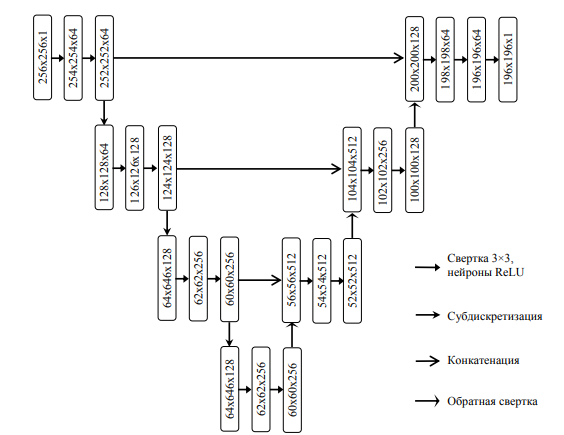
\includegraphics[width=0.50\textwidth]{img/picture_3.png}
            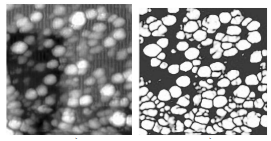
\includegraphics[width=0.30\textwidth]{img/picture_4.png}
        \end{figure}

	\end{frame}

	\begin{frame}\frametitle{}
		\Large
		\center
		\textbf{Спасибо за внимание!}\\
		\vspace{1.5cm}
		\normalsize
		Сажникова О.В.\\
		ПИмд-11\\
		УлГТУ\\
		\vspace{0.5cm}
		\textit{murahika@mail.ru}
	\end{frame}
	
\end{document}

